\documentclass{standalone}
\usepackage{tikz}
\usepackage{amsmath}

\begin{document}

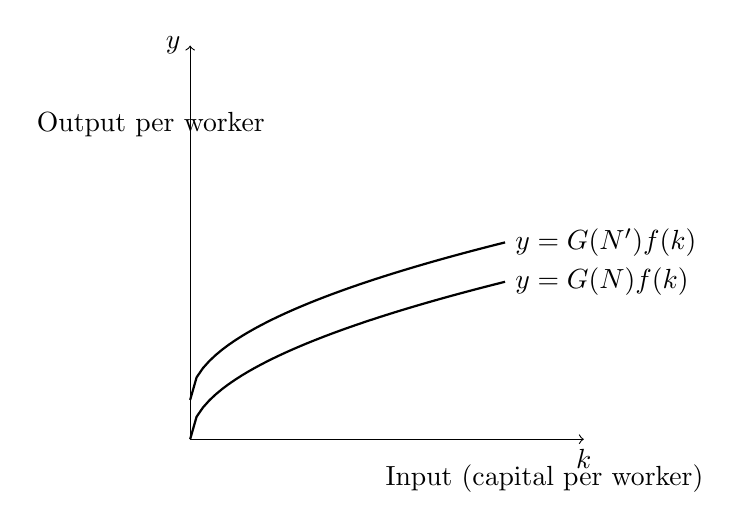
\begin{tikzpicture}
    % Axis
    \draw[->] (0,0) -- (5,0) node[below] {$k$};
    \draw[->] (0,0) -- (0,5) node[left] {$y$};

    % Curves
    \draw[thick] plot[domain=0:4, samples=50] (\x, {sqrt(\x)}) node[right] {$y = G(N)f(k)$};
    \draw[thick] plot[domain=0:4, samples=50] (\x, {sqrt(\x) + 0.5}) node[right] {$y = G(N')f(k)$};

    % Labels
    \node at (-0.5,4) {Output per worker};
    \node at (4.5,-0.5) {Input (capital per worker)};
\end{tikzpicture}

\end{document}